% spline.pic
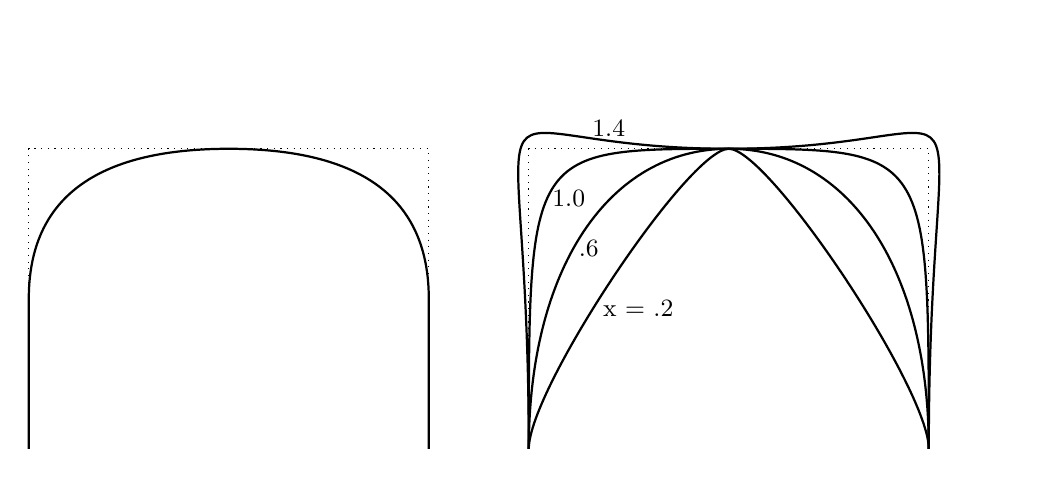
\begin{tikzpicture}[scale=2.54]
% dpic version 2020.03.01 option -g for TikZ and PGF 1.01
\ifx\dpiclw\undefined\newdimen\dpiclw\fi
\global\def\dpicdraw{\draw[line width=\dpiclw]}
\global\def\dpicstop{;}
\dpiclw=0.8bp
\dpicdraw[line width=0.4bp,dotted](0,-0.75)
 --(0,0.75)
 --(2,0.75)
 --(2,-0.75)\dpicstop
\dpicdraw (0,-0.75)
 --(0,0)
 ..controls (0,0.5) and (0.333333,0.75)
 ..(1,0.75)
 ..controls (1.666667,0.75) and (2,0.5)
 ..(2,0)
 --(2,-0.75)\dpicstop
\dpicdraw[line width=0.4bp,dotted](2.5,-0.75)
 --(2.5,0.75)
 --(4.5,0.75)
 --(4.5,-0.75)\dpicstop
\dpicdraw (2.5,-0.75)
 ..controls (2.5,-0.45) and (3.3,0.75)
 ..(3.5,0.75)
 ..controls (3.7,0.75) and (4.5,-0.45)
 ..(4.5,-0.75)\dpicstop
\dpicdraw (2.5,-0.75)
 ..controls (2.5,0.15) and (2.9,0.75)
 ..(3.5,0.75)
 ..controls (4.1,0.75) and (4.5,0.15)
 ..(4.5,-0.75)\dpicstop
\dpicdraw (2.5,-0.75)
 ..controls (2.5,0.75) and (2.5,0.75)
 ..(3.5,0.75)
 ..controls (4.5,0.75) and (4.5,0.75)
 ..(4.5,-0.75)\dpicstop
\dpicdraw (2.5,-0.75)
 ..controls (2.5,1.35) and (2.1,0.75)
 ..(3.5,0.75)
 ..controls (4.9,0.75) and (4.5,1.35)
 ..(4.5,-0.75)\dpicstop
\draw (2.85,-0.05) node[right=-2bp]{\small x = .2};
\draw (2.8,0.25) node{\small .6};
\draw (2.7,0.5) node{\small 1.0};
\draw (2.9,0.85) node{\small 1.4};
\end{tikzpicture}
